For the three algorithms described in Section~\ref{sec:osg-algo}, we developed
implementations in C++ and evaluated them on an Intel Core i7 PC with a 
boost clock of 4.2GHz and 16GiB RAM. For solving ILP models, 
Gurobi solver \cite{optimization2019gurobi} is used. 
%
To evaluate the algorithms, we first generate a set of performance 
benchmarks obtained by subjecting these algorithms through a large set 
of benchmark cases. 
%
Following the synthetic benchmarks, we applied the algorithms on two 
potential application scenarios: guarding the outer perimeter of the 
Warwick Castle and monitoring a building for potential fire eruption 
points.
 
\subsection{Performance Benchmarks}
For creating synthetic benchmarks, to generate the test set $\W$, we 
created simple polygons with the number of vertices ranging between 
$10$ and $200$. 
%
For each instance of the tested polygon, vertices are picked uniform at 
random from $[0,1]\times[0,1]$ and the TSP tour among these vertices are 
used for generating a simple polygon of a reasonable shape.
%
An example is given in ~\ref{fig:osg-ilpexample}.

\def\opgtc{\textsc{Al\_OPG\_2D\_Cont}\xspace}
\def\opgtilp{\textsc{Al\_OPG\_2D\_ILP}\xspace}
\def\orgtilp{\textsc{Al\_ORG\_2D\_ILP}\xspace}
We first evaluate the computational performance of the special \opgt
algorithm where each sensor may cover a single continuous perimeter
segment; denote this algorithm as \opgtc.
%
Table~\ref{tab:osg-opgcont} lists the running time in seconds for 
various $N$ (number of discretized samples) and $k$ (number of guards). 
Various values of $N$ suggest the choices of $\varepsilon$ according to 
the setup of $N$ in Section~\ref{sec:osg-algo}, in this case 
$N=\lceil {len(\partial P)}/{(2\varepsilon)} \rceil$.
Each data point is an average of $100$ examples. As we can observe, the 
method has very good scalability. It also demonstrates the behavior that 
running time is inverse proportional to the number of guards, 
conforming with the statement about time complexity in Section~\ref{subsec:osg-singleseg}. 
% This is due to the larger range of sensing radius that must be searched. In 
% practice, sensing radius is often lower and upper bounded, which means 
% that the algorithm will generally perform better. 
The normalized 
average standard deviation is about $0.06$, which is pretty small. 

\begin{table}[!htbp]
    % \resizebox{1}{1}
    \centering
    \begin{small}
        \begin{tabularx}{0.49\textwidth}{|X|c|c|c|c|c|c|} 
        \hline
        \diagbox{\hspace{1.4mm}$N$\hspace{0.3mm}}{$k$\hspace{0.7mm}} & $5$ & $10$ & $20$ & $30$ & $50$ & $100$ \\
        \hline
        \hspace{5mm}500&0.097 &        0.044 &        0.019 &        0.013 &        0.007 &        0.004 \\
        \hline
        \hspace{5mm}800&0.257 &       0.118 &       0.054 &        0.036 &        0.019 &        0.011 \\
        \hline
        \hspace{4mm}1000&0.385 &       0.183 &       0.082 &        0.055 &        0.029 &        0.016 \\
        \hline
        \hspace{4mm}1500&0.912 &       0.436 &       0.203 &       0.120 &       0.073 &        0.039 \\
        \hline
        \hspace{4mm}2000&1.597 &      0.743 &       0.345 &       0.225 &       0.123 &       0.062 \\
        \hline        
        \end{tabularx}
    \end{small}
    \vspace{0.1in}
    \caption{
        Running time (seconds) for \opgtc.
    }
    \label{tab:osg-opgcont}
\vspace*{-1mm}
\end{table}


Since the $(2 + \varepsilon)$-optimal algorithm is extremely efficient, 
we do not report its running time. For the ILP methods, Table~\ref{tab:osg-opgilp}
and Table~\ref{tab:osg-orgilp} provide the running times for solving \opgt
\begin{table}[htbp]
    % \resizebox{1}{1}
    \centering
    \small{
        \begin{tabularx}{0.49\textwidth}{|X|c|c|c|c|c|c|} 
        \hline
        \diagbox{$GS$}{$k$} & $10$ & $15$ & $20$ & $30$ & $50$ & $100$ \\
        \hline
        \hspace{2.2mm}$50\times 50$   &0.219  &0.127  &0.092  &0.051  &0.023  &0.009\\
        \hline
        \hspace{1mm}$100\times 100$ &0.686  &0.383  &0.250  &0.141  &0.089  &0.033 \\ 
        \hline
        \hspace{1mm}$200\times 200$ &1.915         &1.132         &0.792  &0.444  &0.281  &0.115  \\
        \hline
        \hspace{1mm}$300\times 300$ &7.782         &4.201         &2.613         &1.513         &0.814  &0.435 \\
        \hline
        \hspace{1mm}$400\times 400$ &21.23        &11.63        &7.275         &3.827         &2.231         &1.318 \\        \hline
    \end{tabularx}
    }
    \vspace{0.1in}
    \caption{
        Running time (seconds) for \opgtilp.
    }
    \label{tab:osg-opgilp}
\end{table}
and \orgt, respectively (for convenience, denote these two methods as
\opgtilp and \orgtilp).
Each data point is an average over $10$ cases. 
$GS$ denotes the discrete grid size, suggesting the choice of the grid granularity $\varepsilon$
and the single grid cell size $\varepsilon \times \varepsilon$.
We observe that the ILP method is 
highly effective for solving \opgt and fairly good for solving \orgt. 
The normalized average standard deviation is about $0.125$ for \opgtilp
(which is reasonable) and $0.545$ for \orgtilp (which is relatively large). 

\begin{table}[htbp]
    % \resizebox{1}{1}
    \centering
    \small{
        \begin{tabularx}{0.49\textwidth}{|X|c|c|c|c|c|c|c|} 
        \hline
        \diagbox{$GS$}{$k$} &$10$ & $15$ & $20$ & $30$ & $50$ & $100$ \\
        \hline
        \hspace{2mm}$20\times 20$ &0.252  &0.245  &0.200  &0.170  &0.136  &0.094 \\\hline
        \hspace{2mm}$30\times 30$&1.413 &1.064 &0.886  &0.799  &0.858  &0.576 \\\hline
        \hspace{2mm}$40\times 40$&5.048 &3.598 &3.055 &2.252 &6.114 &1.156 \\\hline
        \hspace{2mm}$50\times 50$ &7.003 &5.617 &4.984 &5.836 &10.91 &0.925\\\hline
        \hspace{2mm}$80\times 80$ &87.14  &84.18   &82.09   &423.5 & $>$2e3 & $>$2e3 \\\hline
        \end{tabularx}
    }
    \vspace{0.1in}
    \caption{
        Running time (seconds) for \orgtilp.
    }
    \label{tab:osg-orgilp}
\end{table}

For solution quality, we compare \opgtc, \opgtilp,
and \orgtilp with the $(2 + \varepsilon)$-optimal solution. For example,
given a test case, let the resulting radius for \opgtc be $r_1$ 
and that for
the $(2+\varepsilon)$-optimal algorithm be $r_2$, we compute the optimality
gain as the reduce of coverage radius over $r_2$ in percentage, 
that is $(r_2 - r_1)/r_2 \cdot 100$. These are then averaged over $10$ cases.
Selected representative results (only three out of a total of 18 rows) are 
given in Table~\ref{tab:osg-comp}. 
In the table, m denotes the method where $\mathbf{1} = $ \opgtc, $\mathbf{2} =$ \opgtilp, 
and $\mathbf{3} = $\orgtilp. Number of samples for \opgtc is set to $2000$. Grid
size for \opgtilp is $200\times 200$. Grid size for \orgtilp is set 
to $40 \times 40$. For each method, we used polygons with $200$ vertices. 
We observe that these algorithms do significantly better than $2$-optimal 
with \opgtilp getting very close to being $1$-optimal (whose optimality gain is
no more than around $50$).

\begin{table}[!htbp]
    % \resizebox{1}{1}
    \centering
    \small{
        \begin{tabularx}{0.485\textwidth}{|c|c|c|c|c|c|c|} 
        \hline
        \diagbox{\,m}{$k$} & $5$ & $10$ & $20$ & $30$ & $50$ & $100$ \\
        \hline
        %\hspace{1.8mm}1 & 10&36.8  &32.9  &33.0  &32.0  &30.2  &29.8  \\\hline
        $\mathbf{1}$ &\,22.34  &\,23.89  &\,27.07  &\,29.14  &\,32.32  &34.18  \\\hline
        %\hspace{1.8mm}2 & 10&47.9  &45.1  &44.3  &42.4  &37.9  &31.9  \\\hline
        $\mathbf{2}$ &\,36.29  &\,34.82  &\,36.22  &\,36.98  &\,37.69  &38.29  \\\hline
        %\hspace{1.8mm}3 & 10&33.8 &28.2 &25.3 &23.0 &19.0 &14.5 \\\hline
        $\mathbf{3}$ &\,35.69 &\,32.58 &\,30.06 &\,25.22 &\,21.99 &15.46\\\hline
        \end{tabularx}
    }
    \vspace{0.1in}
    \caption{ \opgtc, \opgtilp,
and \orgtilp over the $(2 + \varepsilon)$-optimal method.}
    \label{tab:osg-comp}
\end{table}

\subsection{Two Application Scenarios}
Next, we demonstrate the solutions computed by our algorithms on two 
potential application scenarios. For the first one, we apply algorithms
for \opgt on the outer boundary of the Warwick Castle in England (data
retrieved from openstreetmap.org\cite{haklay2008openstreetmap}). ~\ref{fig:osg-wc} shows the 
solution for $15$ guards computed by the $(2 + \varepsilon)$-optimal 
algorithm, \opgtc, and \opgtilp, respectively. Both \opgtc and \opgtilp 
do about $40\%$ better when compared with the $(2 + \varepsilon)$-optimal 
algorithm. \opgtc does $3\%$ better than \opgtilp since the perimeter is 
suitable for continuous guarding while the ILP method is slightly limited
by the chosen resolution.
\begin{figure}[ht]
    \centering
		\small{
	  \begin{overpic}[width=\columnwidth]{chapters/osg/figures/warwick-eps-converted-to.pdf}
        \put(17,-3){(a)}
        \put(50,-3){(b)}
        \put(83,-3){(c)}
    \end{overpic}
		}
		\vspace*{1mm}
    \caption{Solutions for deploying $15$ mobile sensors to guard
		the perimeter of the Warwick Castle. Methods: (a) 
		$(2+\varepsilon)$-optimal. (b) \opgtc. (c) \opgtilp. }
    \label{fig:osg-wc}
\end{figure}

In a second application, we took the footprint of the Brazil 
National Museum and use $40$ mobile robots to monitor it. The solution,
shown in ~\ref{fig:osg-museum}, is computed using \orgtilp. This could be
useful when a building is on fire and drones equipped with heat sensors 
can monitoring ``hot spots'' on top of the building to prioritize fire 
extinguishing effort. There are also many other similar application 
scenarios. 

\begin{figure}[ht]
    \centering
    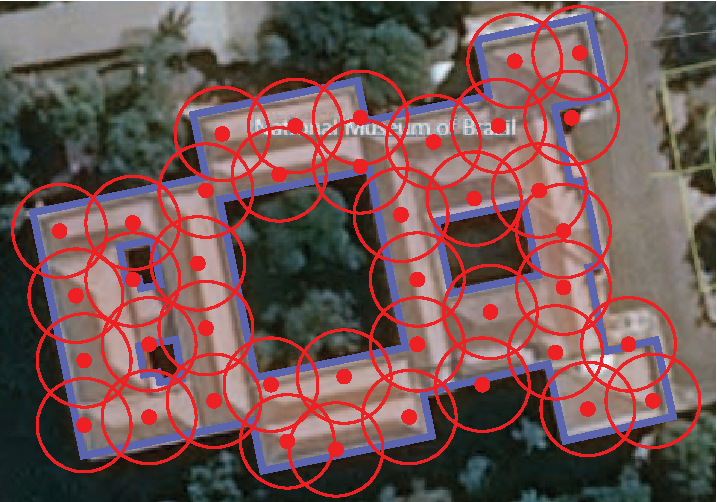
\includegraphics[width=0.95\columnwidth]{chapters/osg/figures/museum-eps-converted-to.pdf}
		\vspace*{1mm}
    \caption{A near-optimal solution for deploying $40$ mobile robots for 
		monitoring the Brazil National Museum, which caught fire in $2019$.}
    \label{fig:osg-museum}
\end{figure}